\section {Central infrastructure}


\subsection {DMWMMON Database as Information store}


\subsection {Data Service as interface to Information store}

\subsection {SiteDb as authentication authority}



\subsection {DashBoard as es end-user visualization tool}

The goal of the visualization is to present the space monitoring information 
in a convenient form, enabling users to check space usage across the sites, 
explore historical views or drill down into a particular directory in the 
CMS storage namespace. While this functionality is required for the central data 
operations and CMS overall storage resource management and utilization, it is
also useful for the site administrators and individual storage users. We opted 
for WLCG Experiment Dashboard \cite{ExpDashboard} framework for the
implementation of space monitoring visualization. CMS dashboard, basd on this 
framework, already provides visualization for monitoring job processing, data 
transfers and site/service usability.

Recently started work with WLCG dashboard developers resulted in the architecture 
proposal shown in Figure 2.
\begin{figure}[h]
\center
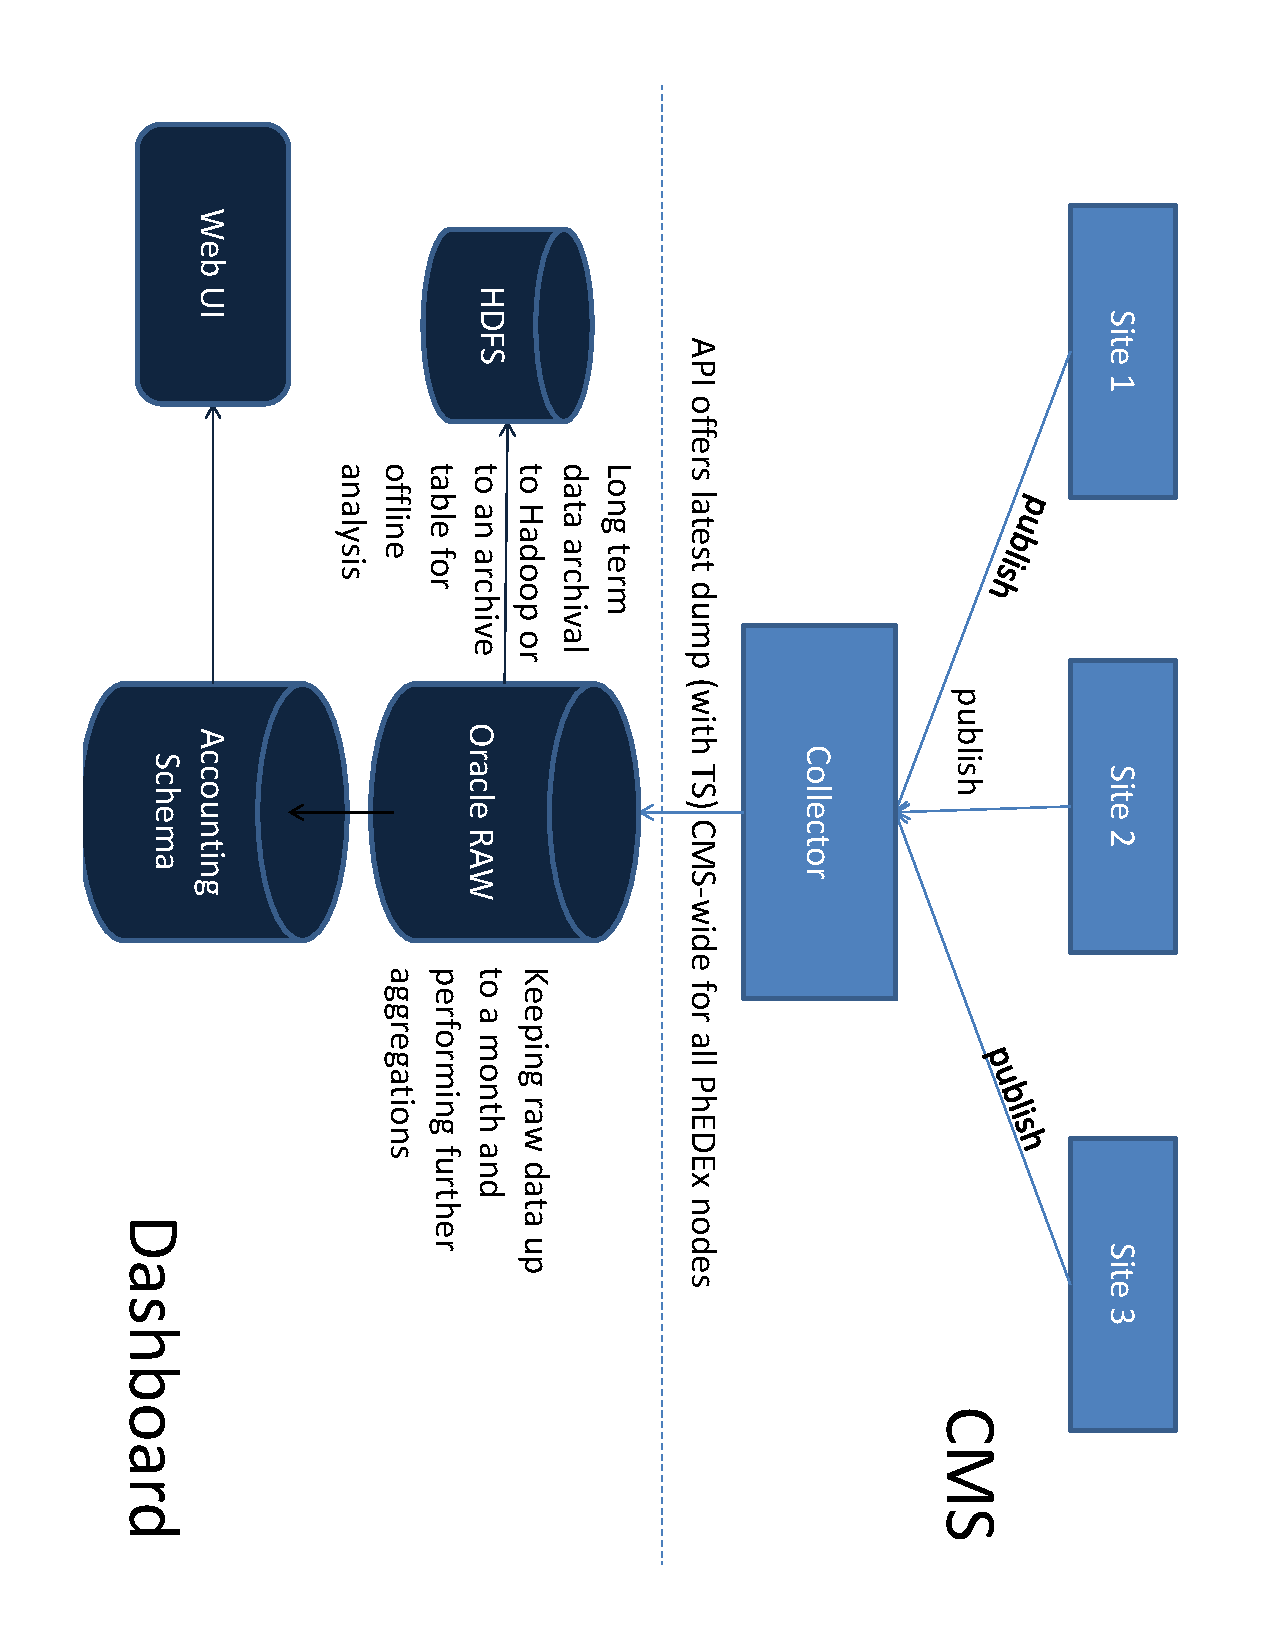
\includegraphics[width=0.8\linewidth, angle =90]
 {pictures/SpaceMonVisProposal-p1.pdf}    
\caption{Proposed architecture for storage accounting and visualization 
in CMS Dashboard based on CMS Space Monitoring information}
\label{fig:vis_proposal}
\end{figure}

Similar design was developed and deployed for monitoring ATLAS space usage 
based on Rucio \cite{Rucio} storage summaries. The challenge in CMS case is to 
represent uniformly the monitoring data asynchronously pushed by the sites.
